\documentclass[times, utf8, seminar, numeric]{fer}
\usepackage[utf8]{inputenc}
\usepackage[T1]{fontenc}
\usepackage{currvita}
\usepackage{graphicx}
\usepackage{epstopdf}
\usepackage{listings}
\usepackage{textcomp}
\usepackage{booktabs}
\usepackage{algorithmic}
\usepackage{algorithm}


% definicija jezika koji nema nista, pa se nista ne naglasava
% koristi se za troadresni kod, ispise tokena i slicno
\lstdefinelanguage{blank}{
	sensitive=false, 
	morecomment=[l]{;},
}

% koristimo zadebljane vektore, a ne strelice
\renewcommand{\vec}[1]{\mathbf{#1}}

% neke boje koje koristimo u formatiranju ispisa
\usepackage{color}
\definecolor{mygreen}{rgb}{0,0.6,0}
\definecolor{mylightgray}{rgb}{0.95,0.95,0.95}

% definicija formatiranja ispisa, ponesto promjenjena u odnosu na pretpostavljenu
\lstset{ %
  backgroundcolor=\color{mylightgray},   % choose the background color; you must add \usepackage{color} or \usepackage{xcolor}
  basicstyle=\footnotesize\ttfamily,        % the size of the fonts that are used for the code
  breakatwhitespace=false,         % sets if automatic breaks should only happen at whitespace
  breaklines=true,                 % sets automatic line breaking
  captionpos=b,                    % sets the caption-position to bottom
  commentstyle=\color{mygreen},    % comment style
  deletekeywords={...},            % if you want to delete keywords from the given language
  escapeinside={\%*}{*)},          % if you want to add LaTeX within your code
  extendedchars=true,              % lets you use non-ASCII characters; for 8-bits encodings only, does not work with UTF-8
  frame=none,                    % adds a frame around the code
  keepspaces=true,                 % keeps spaces in text, useful for keeping indentation of code (possibly needs columns=flexible)
  keywordstyle=\color{blue},       % keyword style
  language=c,           	       % the language of the code
  morekeywords={*,...},            % if you want to add more keywords to the set
  numbers=none,                    % where to put the line-numbers; possible values are (none, left, right)
  numbersep=5pt,                   % how far the line-numbers are from the code
  numberstyle=\tiny\color{gray}, % the style that is used for the line-numbers
  rulecolor=\color{black},         % if not set, the frame-color may be changed on line-breaks within not-black text (e.g. comments (green here))
  showspaces=false,                % show spaces everywhere adding particular underscores; it overrides 'showstringspaces'
  showstringspaces=false,          % underline spaces within strings only
  showtabs=false,                  % show tabs within strings adding particular underscores
  stepnumber=2,                    % the step between two line-numbers. If it's 1, each line will be numbered
  stringstyle=\color{red},     % string literal style
  tabsize=2,                       % sets default tabsize to 2 spaces
  title=\lstname                   % show the filename of files included with \lstinputlisting; also try caption instead of title
}

\title{Implementacija FM-indeks algoritma}

\author{Ivan Borko, Sofia Čolaković, Florijan Stamenković}

\voditelj{doc. dr. sc. Mirjana Domazet Lošo}


\begin{document}

\maketitle

\tableofcontents

\chapter{Uvod i problematika}

Pretraživanje teksta česta je praktična potreba mnogih informacijskih sustava.
Pod terminom "pretraživanje teksta" podrazumijevamo pronalazak svih pojavljivanja
nekog niza znakova $Q$ \engl{query} unutar drugog niza znakova $S$ \engl{string}.
Tipično se rezultat pretraživanja $R$
formulira kao niz indeksa (rednog broja znaka) unutar niza $S$ na kojem počinje pojavljivanje
niza $Q$. Primjerice, za niz $S =$ \textit{"Žuti pas je opasan kad je opasan remenom oko pasa"}
i niz $Q =$ \textit{"pas"} rezultati
pretraživanja su $R = \{6, 14, 28, 46\}$.

U području bioinformatike pretraživanje teksta koristi se u za pronalazak
specifičnih sekvenci unutar zadanog genoma. Definicija pretraživanja je jednaka. Specifičnost
bioinformatičkog pretraživanja jest da su nizovi koji se pretražuju iznimno velike duljine.
Primjerice, ljudski genom tipično sadrži oko $3.3 \times 10^9$ znakova, što bi otisnuto na
A4 stranice fontom veličine 10pt rezultiralo s otprilike milijun stranica.

Postoje mnogi algoritmi pretraživanja teksta
koji na jednostavan način ispunjavaju definirane zahtjeve.
Iz perspektive računalne složenosti algoritama, jednostavno je implementirati pretraživanje
teksta koje radi u linearnom vremenu\footnote{Ako nije drukčije navedeno pri razmatranju složenosti pretraživanja
uvijek govorimo o složenosti s obzirom na duljinu pretraživanog niza $S$.}.
Nažalost, za nizove vrlo velike duljine linearno vrijeme
znači praktično predugo trajanje pretraživanja. Otud potreba, pogotovo u području bioinformatike,
za vremenski sub-linearnim algoritmima pretraživanja.

U ovom projektu razmatramo implementaciju pretraživanja teksta koja se bazira na konceptu
FM-indeksa. Konkretna implementacija bazira se na binarnim stablima valića \engl{wavelet-trees}.
Teoretsko razmatranje i praktično testiranje pokazuju da ovakva implementacija pretraživanja
ima vremenski sub-linearnu složenost.

\chapter{FM-indeks algoritam}

"Indeksiranje" teksta označava generiranje struktura podataka koje su podrška efikasnom
pretraživanju. Za velike tekstove poželjno je da indeks bude memorijski efikasan.
FM-indeks \cite{Ferragina00opportunisticdata} pristup je indeksiranju koji ispunjava
zahtjeve memorijske efikasnosti i sub-linearnog vremena pretraživanja. Prije nego definiramo
FM-indeks, potrebno je razmotriti podatkovne strukture i algoritme koji ga sačinjavaju.

\section{Burrows-Wheeler transformacija (BWT)}

Burrows-Wheeler transformacija \cite{btw_1994} transformira niz znakova na način koji
će omogućiti efikasnu pohranu i brzo ptreživanje. BWT transformirani niz originalnog
teksta $T$ označavati ćemo sa $T^{BTW}$. Transformacija se provodi sljedećim koracima:

\begin{enumerate}
  \item{Poseban znak $\$$ koji je leksikografski manji od svih ostalih znakova se dodaje na kraj niza $T$}
  \item{Cikličkim rotacijama niza $T$ dobiva sa se skup nizova koji čini tablicu $CR$ \engl{cyclic rotation}}
  \item{Tablica $CR$ se leksikografski sortira u tablicu $SRC$}
  \item{Posljednji stupac tablice $SCR$ se ektrahira u rezultat $T^{BTW}$}
\end{enumerate}

Opisani postupak ilustriran je za niz \textit{T = "AGATTAT"} na slici \ref{fig:bwt}, preuzetoj iz rada
\cite{singer_2012}.

\begin{figure}[!htb]
\centering
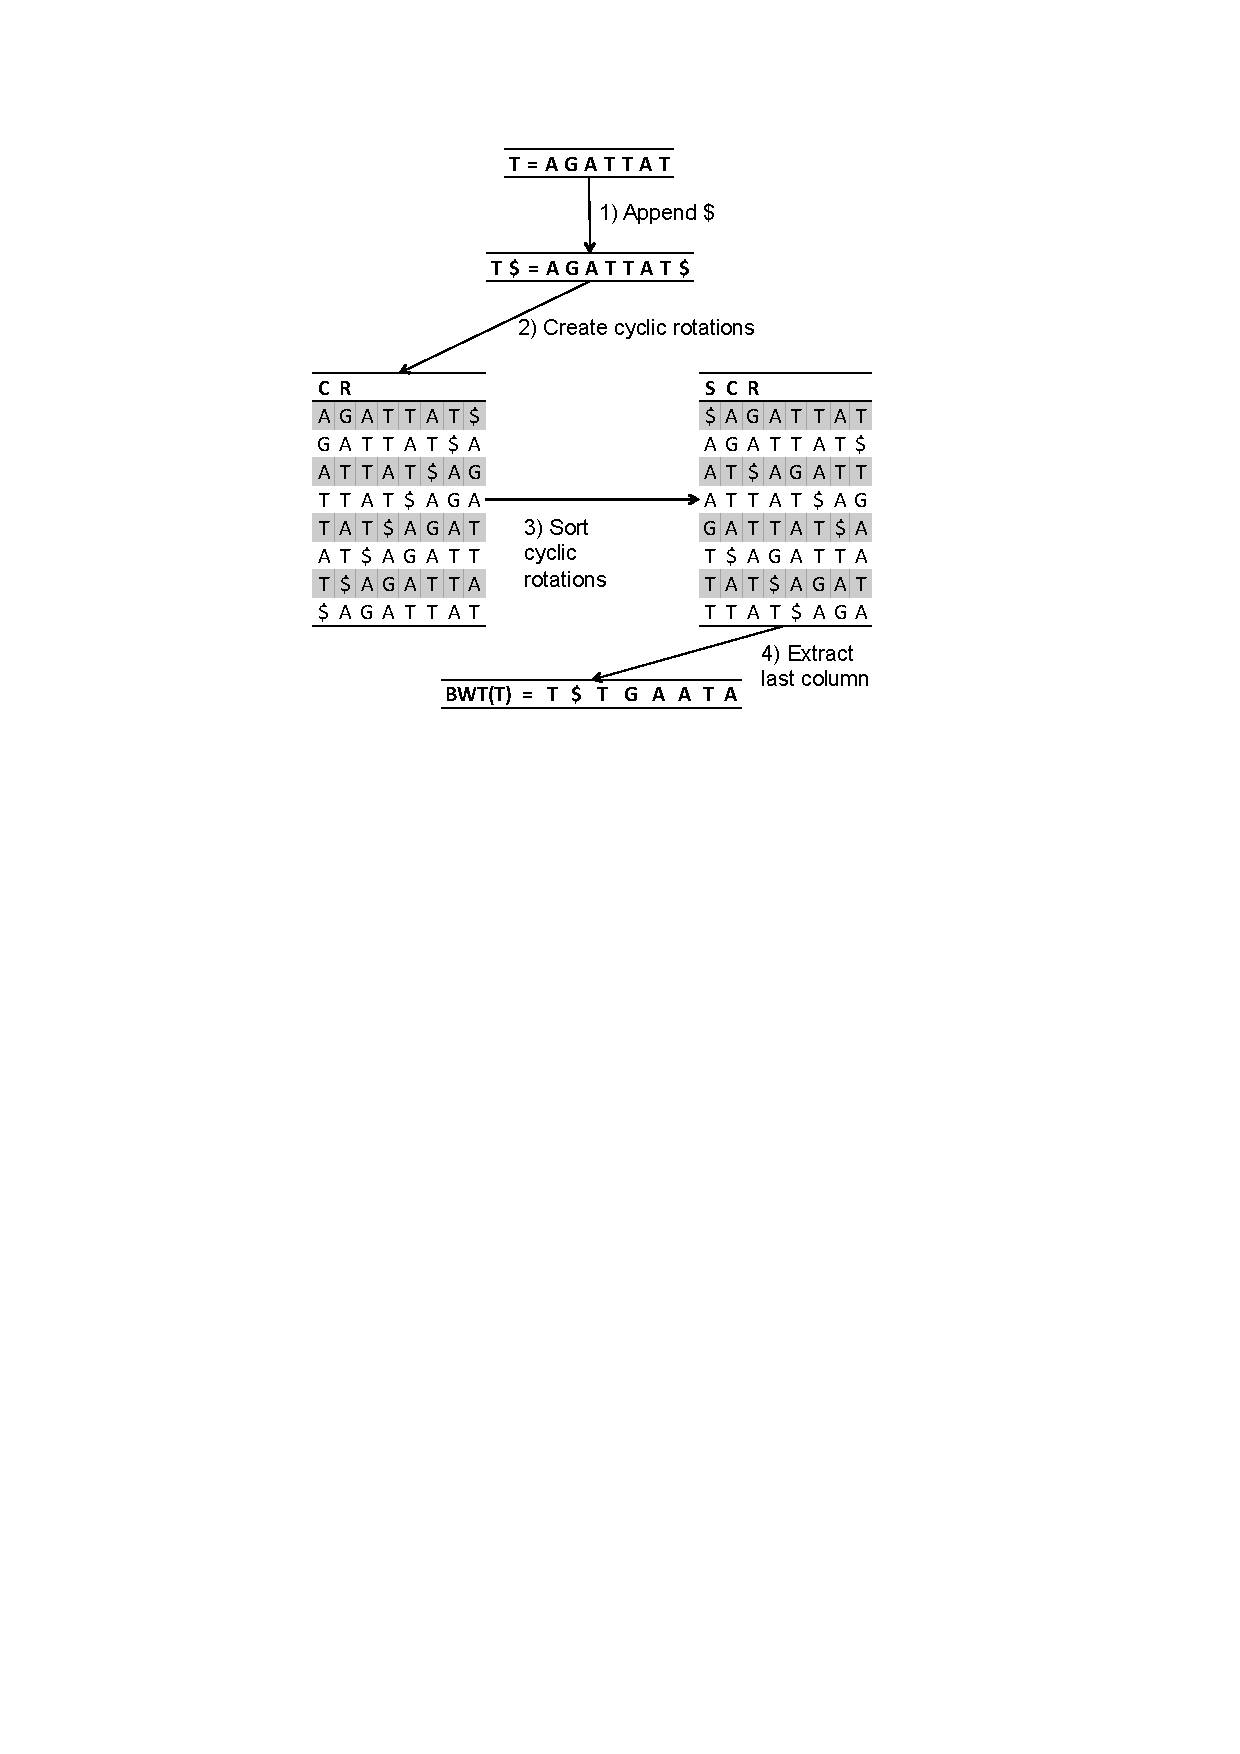
\includegraphics{fig/bwt.pdf}
\caption{Primjer algoritma BWT transormacije niza \textit{T = AGATTAT}}
\label{fig:bwt}
\end{figure}

Bitno je primjetiti kako je BWT transformacija niza srodna sufiksnoj listi $SA$ \engl{suffix array}. Sufiksna lista
je struktura podataka koja se često koristi u algoritmima nad tekstom. Njenu formulaciju
nećemo detaljno objašnjavati, materijali na temu su široko dostupni. Sličnost između BWT
transformacije i $SCR$ tablice korištene u BWT transformaciji ilustrirana je slikom \ref{fig:bwt_sa}.

\begin{figure}[!htb]
\centering
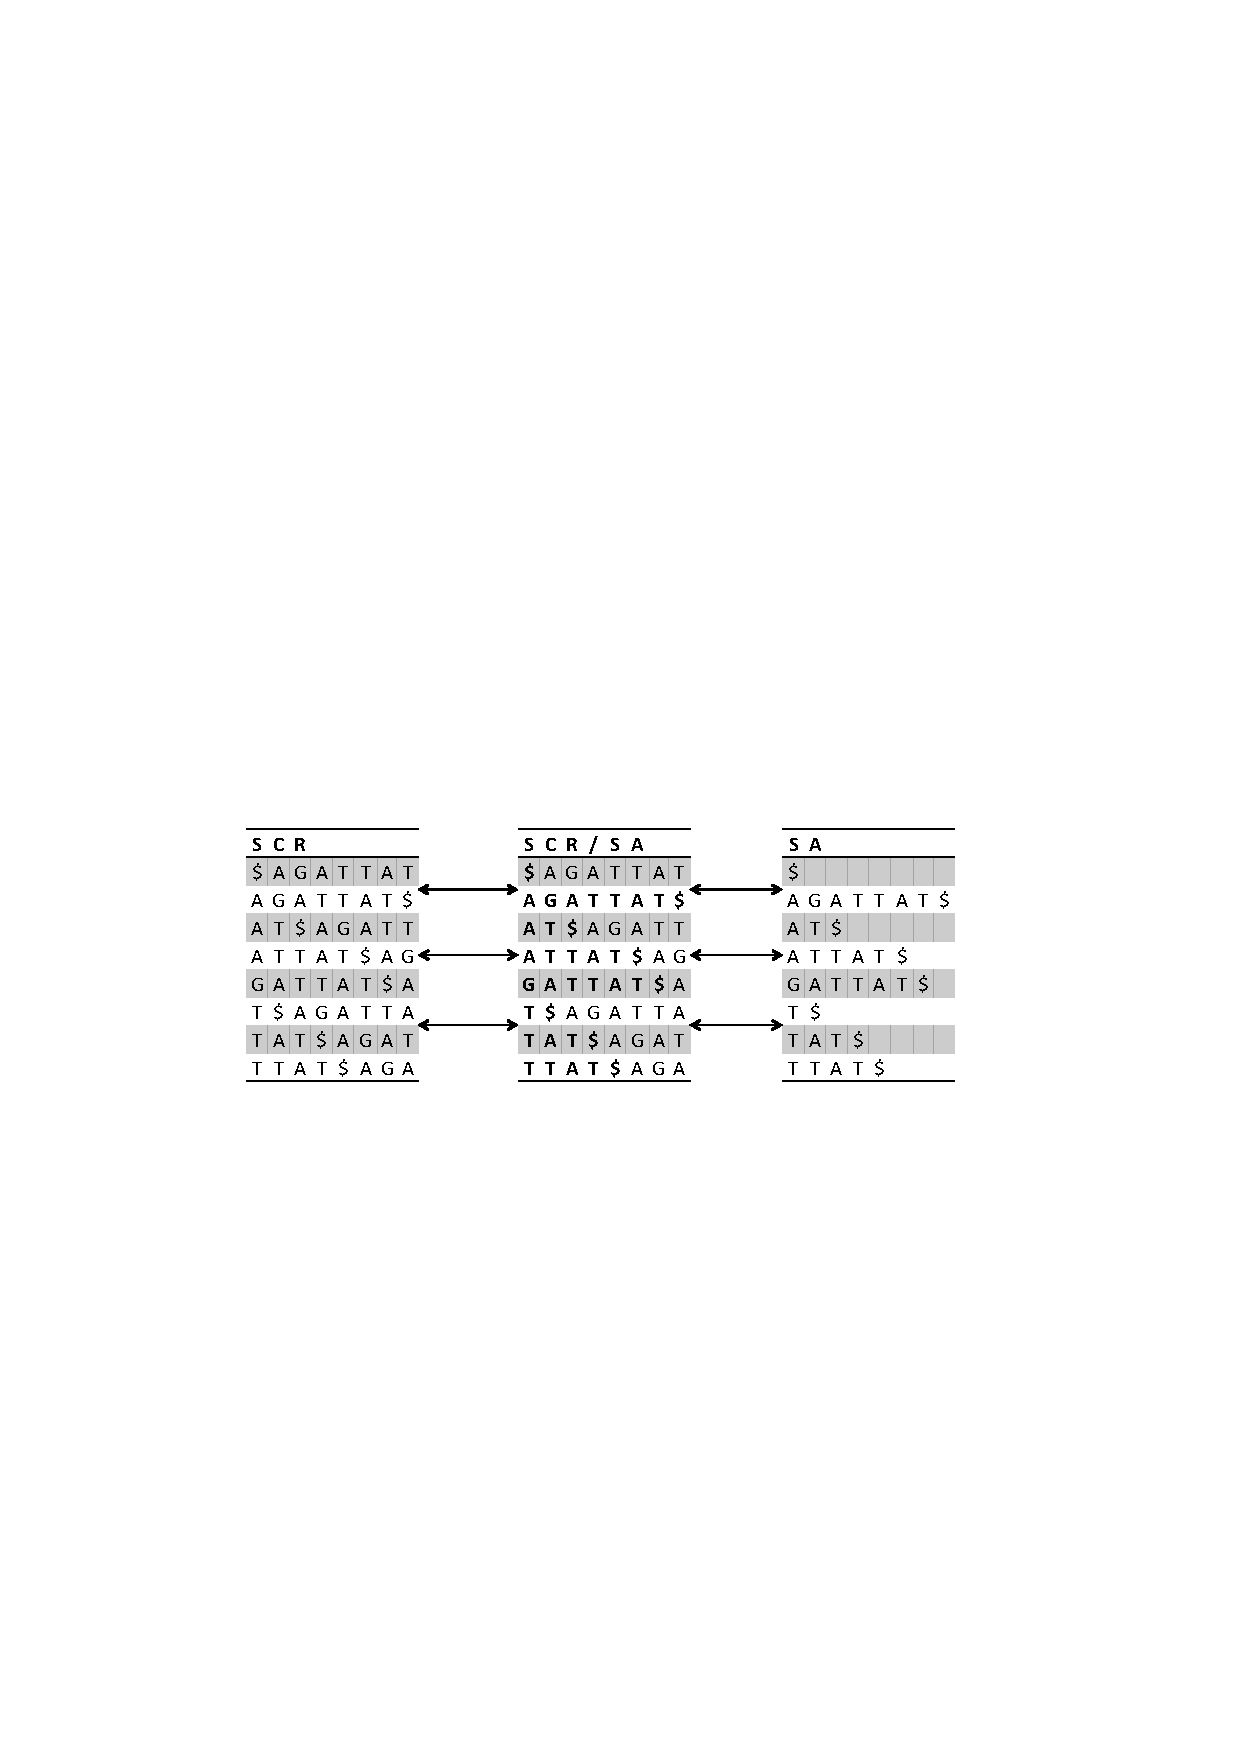
\includegraphics{fig/bwt_sa.pdf}
\caption{SCR tablica BWT tranfsformacije i sufiksna lista za niz \textit{T = AGATTAT}}
\label{fig:bwt_sa}
\end{figure}


\chapter{Implementacija i testiranje}

\chapter{Zaključak}
Zaključak.

\bibliography{literatura}
\bibliographystyle{unsrt}

\chapter{Sažetak}
Sažetak.

\end{document}
